\documentclass[solution,addpoints,12pt]{exam}
\printanswers
\usepackage{amsmath,amssymb,graphicx}
\usepackage{centernot}
\usepackage{hyperref}
\usepackage{bbm}
\usepackage{amsfonts}
\newcommand{\RP}{\ensuremath{\mathsf{RP}}}
\newcommand{\expect}[1]{\ensuremath{\mathbb{E}[#1]}}
\newcommand{\dx}{\mathrm{d}x}
\newcommand{\real}{\mathbb{R}}
\usepackage{graphicx}
\graphicspath{ {./images/} }
\hypersetup{
    colorlinks=true,
    linkcolor=blue,
    filecolor=magenta,      
    urlcolor=cyan,
}

%\documentclass[addpoints,11pt,a4paper]{exam}
\renewcommand{\rmdefault}{ppl} % rm
\linespread{1.05}        % Palatino needs more leading
\usepackage[scaled]{helvet} % ss
\usepackage{courier} % tt
\usepackage{eulervm} % a better implementation of the euler package (not in gwTeX)
\normalfont
\usepackage{caption}
\usepackage[T1]{fontenc}
\usepackage{mathrsfs}
\usepackage{comment}
\usepackage{graphicx}
\usepackage{ulem}
\usepackage{paralist}
\usepackage{amsmath}
\usepackage{psfrag}
\usepackage{fullpage}
\usepackage{fancybox}
\usepackage{ifthen}
\usepackage{hyperref}
\usepackage{float}
\usepackage{listings}             % Include the listings-package
\newcommand{\red}[1]{\textcolor{red}{#1}}
%commands added



%%%%%%%%%%%%%%%%%%%%%%%%%%%%%%%%%%%%%


\lstset{language=Python}
\usepackage{marvosym}
\usepackage[export]{adjustbox}
\extrawidth{1in}
\usepackage{multicol}
\setlength{\columnsep}{.001cm}
\newcommand{\twopartdef}[4]
{
	\left\{
		\begin{array}{ll}
			#1 & \mbox{if } #2 \\
			#3 & \mbox{if } #4
		\end{array}
	\right.
}
\newcommand{\G}{\mathcal{G}}
\newcommand{\fH}{\mathcal{H}}
\newcommand{\M}{\mathcal{M}}

\begin{document}

\hrule
\vspace{3mm}
\noindent 
{\sf IITM-CS5691 : Pattern Recognition and Machine Learning  \hfill Release Date: Sep 28, 2021}
\\
\noindent 
{\sf Assignment 1 (MKN Section) \hfill Due Date : Oct 7, 23:59}
%{\sf ~\hfill }
\vspace{3mm}
\hrule
\vspace{3mm}
\noindent{{\sf Roll No: CS19B015}  \hfill  {\sf Name: Challa Sai Shashank Reddy}}\\% put your ROLL NO AND NAME HERE
\noindent{{\sf Roll No:CS19B024}  \hfill  {\sf Name: Konthalapalli Abhishek}}% put your ROLL NO AND NAME HERE

\noindent
{{\sf Team number: }} %Team number

\noindent
{{\sf References (if any): 
}} %Reference materials, if any.


\vspace{3mm}
\hrule
{\small
\begin{itemize}\itemsep0mm
\item This assignment has to be completed in teams of two. Collaborations outside the team are strictly prohibited.
\item Use \LaTeX\ to write-up your solutions (in the solution blocks of the source \LaTeX\  file of this assignment), and submit the resulting single pdf file at GradeScope by the due date. (Note: {\bf No late submissions} will be allowed, other than one-day late submission with 10\% penalty or four-day late submission with 30\% penalty! Within GradeScope, indicate the page number where your solution to each question starts, else we won't be able to grade it! You can join GradeScope using course entry code {\bf N8Z67W})  
\item For the programming questions, please submit your code directly in moodle (carefully following the filename/folder/README conventions given in the questions/moodle), but provide your results/answers in the pdf file you upload to GradeScope. We will run plagiarism checks on codes, and any detected plagiarism in writing/code will be strictly penalized. 
% mvoe to moodle: Attach a \textbf{README} with your code submission which gives a brief overview of your approach and a single command-line instruction for each question to read the data and generate the test results and figures. 
\item  If you have referred a book or any other online material for obtaining a solution, please cite the source. Again don't copy the source {\it as is} - you may use the source to understand the solution, but write-up the solution in your own words. 
\item Points will be awarded based on how clear, concise and rigorous your solutions are, and how correct your code is. Overall points for this assignment would be ${\bf min}$(your score including bonus points scored, 50).
\item Check the Moodle discussion/announcement forums regularly for updates regarding the assignment. Please start early and clear all doubts ASAP. Post your doubt only on Moodle Discussion Forum so that everyone is on the same page. Please note that the TAs can \textbf{only} clarify doubts regarding problem statements (they won't discuss any prospective solution or verify your solution or give hints). 
\end{itemize}
}
\hrule


\begin{questions} 
\question[15] [{\sc Density Estimation}]
\begin{parts}
\part[5] [{\sc Parametric MLE}]
Suppose that the lifetime of Philips brand light bulbs is modeled by an exponential distribution with (unknown) rate parameter $\lambda$ or alternatively mean parameter $\mu$. We test 6 bulbs and find they have lifetimes of 2, 6, 7, 1, 4, and 3 years, respectively. (i) (2 points) What is the MLE for $\lambda$ and for $\mu$, and (ii) (2 points) derive the bias of each of these estimators? (iii) (1 point) If the estimators are biased, how will you correct them to get unbiased estimators?
\begin{solution}

This is MLE of $\lambda\mid\mu$ of exponential distribution $\lambda e^{-\lambda x}$

\begin{align*}
    \lambda_{ml} &= \operatorname*{argmax}_\lambda  \prod_{i=1}^{n} P(x_i;\lambda) \\ 
    &=\operatorname*{argmax}_\lambda  \prod_{i=1}^{n} \lambda e^{-\lambda x_i} \\ 
    &= \operatorname*{argmax}_\lambda \sum_{i=1}^{n} (\log{\lambda} - \lambda x_i) \\ 
    &= \operatorname*{argmax}_\lambda (n\log{\lambda} - \lambda \sum_{i=1}^{n} x_i)
\end{align*}

Differentiating this expression which respect to $\lambda$ we get, 
\begin{align*}
    \frac{n}{\lambda} - \sum_{i=1}^{n} x_i = 0  \\ 
    \lambda = \frac{n}{\sum_{i=1}^{n} x_i},   
    \mu_{ml} = \frac{1}{\lambda_{ml}} = \frac{\sum_{i=1}^{n} x_i}{n} \\
\end{align*}

%  

\end{solution}

\part[5] [{\sc Parametric Bayesian}] Assume we have following prior distribution on $\theta$:
$$p(\theta) = \alpha\beta^{\alpha}\theta^{-\alpha-1} \mathbbm{1}_{(\beta,\infty)} (\theta)$$
where $\mathbbm{1}_{(\beta,\infty)} (\theta)$ is an indicator function which equals 1 when $\beta <\theta < \infty$ and $0$ otherwise.
$p(\theta)$ is called Pareto distribution which is denoted as $\theta \sim $
Pareto$(\alpha, \beta)$.
\begin{subparts}
\subpart[1\half] Assume $\theta \sim $
Pareto$(\alpha, \beta)$ and $X_1,\dots , X_n \sim $ Uniform$(0, \theta)$ which are conditionally
independent given $\theta$. What is the posterior distribution $p(\theta|D)$ where $D=(x_1,x_2,\dots,x_n)$. Does it belong to any family of distributions that you recognize?
\begin{solution}
% \[
%     \begin{cases}
    
%     \end{cases}

% \]
\[ p(\theta)=  
    \begin{cases} 
      0 & \theta\leq \beta \\
      \alpha\beta^{\alpha}\theta^{-\alpha-1} & \beta < \theta < \infty 
    \end{cases}
\]

\begin{align*}
    p(\theta|D) = \frac{p(D|\theta)p(\theta)}{p(D)} \\ \\  
    \text{Now,} \ \bar{\beta} = max(x_1,x_2 \ldots x_n) \\ 
    = \frac{\frac{1}{\theta^(n)}\alpha\beta^{-\alpha-1}}{    \int_{\bar{\beta}}^{\infty}\frac{\alpha\beta^{\alpha}\theta^{-\alpha-1}}{\theta^{n}} d\theta}  
    &= \frac{\theta^{-\alpha-n-1}}{\int_{\widetilde{\beta}}^{\infty}\theta^{-\alpha-n-1}d\theta} \\ 
    \int_{\widetilde{\beta}}^{\infty}\theta^{-\alpha-n-1}d\theta = \frac{\widetilde{\beta}^{-\alpha-n}}{\alpha+n} \\
    \frac{\theta^{-\alpha-n-1}}{\int_{\widetilde{\beta}}^{\infty}\theta^{-\alpha-n-1}d\theta} = \frac{-\theta^{\alpha -n-1} \times (\alpha + n)}{\widetilde{\beta}^{-\alpha-n}} \\ 
    &= (\alpha +n)\widetilde{\beta}^{\alpha+n}\theta^{-(\alpha+n)-1} \\ 
    &= \text{pareto}(\alpha+n, \widetilde{\beta})
    % \int_{\beta}^{\infty}\theta^{-\alpha-n-1}d\theta = \frac{\beta^{}}{} 
\end{align*}


\end{solution}

\subpart[1\half] Using the above derived posterior, calculate the MAP estimate of $\theta$? How does this compare to the MLE?
\begin{solution}

The likelihood is :  
\[
  P(D;\theta) = \frac{1}{\theta^{n}}
\]
MLE estimate would be $\theta = max(x_1, x_2, x_3, \ldots x_n)$
The pareto function is a strictly decreasing function from $\theta \geq \widetilde{\beta}$, 
therefore the MAP estimate of this would be $\widetilde{\beta}$. 

Therefore both the MLE estimate and MAP estimate of $\theta$ would be the same.  

\end{solution}

\subpart[2] Square loss is defined as $L(\theta, \hat{\theta}) = (\theta - \hat{\theta})^2$. For the above derived posterior in (i), 
what estimator of $\theta$ minimizes the posterior expected square loss? Simplify your answer as much as possible. Is it the same as the MLE and/or the MAP?
\begin{solution}

To minimize  $L(\theta, \hat{\theta}) = (\theta - \hat{\theta})^2$ we have to minimize $E[(\theta - \hat{\theta})^{2}]$ 
\[
  \int_{-\infty}^{\infty} (\theta - \hat{\theta})^2 p(\theta)d\theta 
\]

\begin{align*}
  \int_{-\infty}^{\infty} \theta^{2} p(\theta) d\theta -  2\int_{-\infty}^{\infty} \theta \hat{\theta} p(\theta) d\theta + \int_{-\infty}^{\infty} \hat{\theta}^2 p(\theta) d\theta 
\end{align*}

\[
  \int_{-\infty}^{\infty} \theta^{2} p(\theta) d\theta -  2 \hat{\theta} E[\theta] + \hat{\theta}^2 p(\theta) 
\]
Now differentiating by $\hat{\theta}$ we get, 

\[
  2\hat{\theta} = 2E[\theta]  
\]
\[
  \hat{\theta} = E[\theta]
\]

This function would reach it's minimum value when $\theta$ takes the value $E[\theta]$. 
Expectation of $\theta$ is as follows:

\begin{align*}
  E(\theta) = \int_{\beta}^{\infty} \theta \alpha \beta ^{\alpha}\theta^{-\alpha-1} d\theta \\ 
  &= \alpha\beta^{\alpha} \int_{\beta}^{\infty} \theta^{-\alpha} d\theta \\ 
  &= \alpha \beta^{\alpha} \left[ \frac{\theta^{\alpha-1}}{-\alpha +1} \right]^{\infty}_{\beta}
\end{align*}
Which is equal to, \\ 

\[  
  E[\theta] = \begin{cases}
      \infty &  \alpha <= 1  \\ 
      \frac{\alpha \beta}{\alpha-1} & \alpha > 1 \\
  \end{cases}
\]

Therefore $\hat{\theta}$ is equal to, 
\[  
  \hat{\theta} = \begin{cases}
      \infty &  \alpha <= 1  \\ 
      \frac{\alpha \beta}{\alpha-1} & \alpha > 1 \\
  \end{cases}
\]


\end{solution}
\end{subparts}

\part[5] [{\sc Non-parametric method}]
In class, we saw a Parzen window estimator using an unit hypercube as the Parzen window or kernel function; we will use an exponential kernel function here:  
\begin{gather*}
  k(u)=
    \begin{cases}
    e^{-u}\quad u > 0, \\
    0  \quad \quad u\leq 0.
    \end{cases}
\end{gather*}
If $D=\{x_1,x_2 \cdots x_n\}$ is a dataset of i.i.d. samples, each drawn from $U(0,1)$, then (i) (3 points) show that the mean of the estimated density $p(x)$ is given by: 
\[
E_D[p(x)]=
\begin{cases}
0\quad \quad \quad \quad \quad x <0\\~\\
{1-e^{-\dfrac{x}{h}}}\quad \quad \quad 0\leq x\leq 1\\~\\
{e^{\dfrac{1-x}{h}} - ~e^{-\dfrac{x}{h}}}\quad \quad x \geq 1.
\end{cases}
\]
(ii) (2 points) Also, plot $E_D[p(x)]$ vs $x$ for different values of $h$ ($h=1, 0.25, \mathrm{~and~} 0.0625$). What do you observe?
\begin{solution}
%insert the solution here
\end{solution}
\end{parts}


\question[10] [{\sc Bayesian Decision Theory}]
\begin{parts}
\part[5][Optimal Classifier by Pen/Paper]
Let $L$ be the loss matrix defined by $L=\begin{bmatrix}
 0 &1 &2\\
 1 &0 &1\\
 2 &1 &0
\end{bmatrix}$, where $L_{ij}$ indicates the loss for an input x with $i$ being the true class and $j$ the predicted class. Given the data:
\begin{center}
    \begin{tabular}{|c|c|c|c|c|c|c|c|c|c|c|c|c|c|c|c|c|c|}
    \hline
    \textbf{x} &-2.9 & 1.4 & 0.4 &-0.3 & -0.7 & 0.9 & 1.8 & 0.8 & -2.4 & -1.4 & 1.2 & 2.3 & 2.8 & -3.4\\
    \hline
     \textbf{y}& 1 & 3 & 2 & 2 & 1 & 3 & 3 & 2 & 1 & 1 & 2 & 3 & 3 & 1\\
     \hline
\end{tabular}
\end{center}
find the optimal Bayes classifier $h(x)$, and provide its decision boundaries/regions. 
\begin{solution}




% \begin{align*)
%   P_{X|Y=1} = N(\mu_1, I), P(Y=1) = \phi_1 \\  
%   P_{X|Y=2} = N(\mu_2, I), P(Y=1) = \phi_2 \\ 
%   P_{X|Y=3} = N(\mu_3, I), P(Y=1) = \phi_3 \\ 
% \end{align*}

\begin{align*}
    P_{X|Y=1} = N(\mu_1, I), P(Y=1) = \phi_1 \\  
  P_{X|Y=2} = N(\mu_2, I), P(Y=1) = \phi_2 \\ 
  P_{X|Y=3} = N(\mu_3, I), P(Y=1) = \phi_3 \\ 
\end{align*}
Now through MLE estimation
\[
  \operatorname*{argmax}_{\mu_1,\mu_2, \mu_3, \phi_1, \phi_2, \phi_3} \prod_{i=1}^{n} P(x_{i}| y_{i})p(y_{i})
\]
Solving this problem we would get, 

\[
  \mu_i = \frac{\sum_{j=1}^{n}x_j \mathbbm{1}{y_j = i}}{ \sum_{j=1}^{n} \mathbbm{1}{y_j = i} }
  \phi_i = \frac{\sum_{i=1}^{n}\mathbbm{1}{y_j = i}}{n}
  \sigma_i = \frac{\sum_{j=1}^{n} (x_j - \mu_j)^2 \mathbbm{1}{y_j = i}}{\sum_{j=1}^{n} \mathbbm{1}{y_j = i}}
\]

\begin{align*}
  \mu_1 = \frac{-2.9 -0.7 -2.4 -1.4-3.4}{5} = -2.16 \\ 
  \mu_2 = \frac{0.4+0.3-0.3+1.2}{4} = 0.525 \\ 
  \mu_3 = \frac{1.4+0.9+1.8+2.3+2.8}{5} = 1.84 
\end{align*}
\begin{align*}
  \phi_1 = \frac{5}{14} \\ 
  \phi_2 = \frac{4}{14} \\ 
  \phi_3 = \frac{5}{14}
\end{align*}

for optimal bayes classifier 

Now to calculate the posterior expressions, 
\[
  t = \begin{bmatrix}
    t_1 \\ 
    t_2 \\ 
    \vdots \\ 
    t_N 
    \end{bmatrix} 
\]

\[
\text{let }p = \begin{bmatrix}
  p(x|y=1) \\ 
  p(x|y=2) \\ 
  p(x|y=3)
\end{bmatrix}
\]
And loss function for each class be  $L(t = C_1), L(t = C_2), L(t = C_3)$ 
\[
\begin{bmatrix}
  L(t=C_1) \\ 
  L(t=C_2) \\ 
  L(t=C_3)
\end{bmatrix}
= 
\begin{bmatrix}
  0&1&2 \\ 
  1&0&1 \\ 
  2&1&0 \\ 
\end{bmatrix}
\begin{bmatrix}
  p(C_1|x)\\
  p(C_2|x)\\ 
  p(C_3|x)\\ 
\end{bmatrix}
\]  

\[
\begin{bmatrix}
  L(t=C_1) \\ 
  L(t=C_2) \\ 
  L(t=C_3)
\end{bmatrix}
= 
\begin{bmatrix}
  p(C_2|x) +2p(C_3|x) \\
  p(C_1|x) + p(C_3|x)\\ 
  2p(C_1|x) + p(C_2|x)\\ 
\end{bmatrix}
\]  

\[
\begin{bmatrix}
  L(t=C_1) \\ 
  L(t=C_2) \\ 
  L(t=C_3)
\end{bmatrix}
= 
\begin{bmatrix}
  N(1.46,0.2720) \\
  N(-0.32, 0.1802)\\ 
  N(-1.39,0.5414)\\ 
\end{bmatrix}
\]  
\[
  h(x) = \operatorname*{argmin}_{C_k} L(t = C_k), \text{for k =1,2,3}   
\]

On comparing the log of the loss functions and solving we get the decision boundaries as, 

\[
  h(x) = \begin{cases}
    C_1 & x_1 \le -0.512 \\ 
    C_2 & -0.512 < x \le 1.111 \\ 
    C_3 & x > 1.111
  \end{cases}
\]


\end{solution}

\part[5]
Consider the problem of  classifying a pattern $x$ into one of the $k$ classes $c={1, 2, ...k}$. Assume that we have two different tests to determine the class to be assigned to pattern $x$. Test 1 assigns $x$ to the class that maximizes the posterior probability, whereas test 2 to a class chosen based on randomized decision rule.
\begin{center}
\begin{tabular}{l}
Test 1:   $H_1(x) = c^* = \operatorname*{argmax}_{c} p(c|x)$ \\

Test 2:   $H_2(x) = c \sim p(c|x)$, where $c$ is chosen based on the distribution\\ $P(c=i|x)$ in a random fashion.
\end{tabular}
\end{center}
\begin{subparts}
\subpart[1] Calculate the risk $\mathrm{R_1}$ associated with test 1 in terms of the posterior probability using the zero-one loss function.
\begin{solution}
  \begin{align*}
    Loss(c_1 , c_2) =\begin{cases}
        0 & c_1 = c_2 \\ 
        1 & c_1 \neq c_2 
    \end{cases} \\ 
    R_1 = \operatorname*{E[L(c,c^{*})]}_{c\sim p(c|x)}= \sum_{i=1}^{k}L(c,c^{*})p
    &= 1- p(c^{*}|x)
  \end{align*}
\end{solution}

\subpart[2] Calculate the risk $\mathrm{R_2}$ associated with test 2 in terms of the posterior probability using the zero-one loss function.
\begin{solution}
  \begin{align*}
    Loss(c_1 , c_2) &=\begin{cases}
        0 & c_1 = c_2 \\ 
        1 & c_1 \neq c_2 
    \end{cases} \\ 
    R_1 = \operatorname*{E[L(c,c^{*})]}_{c\sim p(c|x)c^{*} \sim p(c|x)} &= \sum_{j = 1}^{k}\sum_{i=1}^{k}L(i,j)p(c = i|x)p(c^{*} = j|x) \\
    &= \sum_{j=1}^{k}(1 - p(c^{*} = j|x)) p(c^{*} = j|x) \\
    &=  \sum_{j=1}^{k}p(c^{*} = j|x) - \sum_{i=1}^{k}(p(c^{*} = j|x))^{2}  \\
    &= 1 - \sum_{j=1}^{k}(p(c^{*} = j|x))^{2} 
  \end{align*}
\end{solution}

\subpart[2] Which test do you think would perform better always based on the risks $R_1$ and $R_2$? Also, specify the conditions under which both the tests behave the same.
\begin{solution}

  $R_1$ is better than $R_2$   
  \begin{align*}
    R_1 = R_2 \text{ if }  P(c^{*}|x) = 1 \text{ and all other} P (c_i|x) =0
  \end{align*}
  
\end{solution}
\end{subparts}
\end{parts}


\question[15][Linear regression] 
\begin{parts}
\part[5] Say we have a linear regression dataset where every training datapoint $\{x_n,y_n\}$ has a weight $q_n$ ($q_n > 0$) identified with it. Then we have the weighted error function (sum of squares) given by: 
\[
E_q(w)=\sum_{n=1}^{N} \dfrac{q_n(t_n - w^T x_n)^2}{2}.
\]
Derive the closed form solution for the minimizer $w^{*}$ of this function. Express it in matrix format for a simplified expression. 
\begin{solution}
% \beta + \alpha  = x+y +z  
\[
  E_q(w)=\sum_{n=1}^{N} \frac{((q_n)^{1/2}t_n - (q_n)^{1/2}w^T x_n)^2}{2}
\]
\[
  t = \begin{bmatrix}
  t_1 \\ 
  t_2 \\ 
  \vdots \\ 
  t_N 
  \end{bmatrix} 
  \quad \quad \quad
  t_q = \begin{bmatrix}
    t_{1}(q_{1})^{1/2} \\ 
    t_{2}(q_{2})^{1/2} \\ 
    \vdots \\ 
    t_{N}(q_{N})^{1/2} 
    \end{bmatrix} 
\]

\[
  x_n  = \begin{bmatrix}
  x_n^{(1)} \\ 
  x_n^{(2)} \\ 
  \vdots \\ 
  x_n^{(D)} 
  \end{bmatrix} 
  \quad \quad \quad
  x_{nq} = \begin{bmatrix}
    x_n^{(1)}(q_{n}^{(1)})^{1/2} \\ 
    x_n^{(2)}(q_{n}^{(2)})^{1/2} \\ 
    \vdots \\ 
    x_n^{(D)}(q_{n}^{(D)})^{1/2}
    \end{bmatrix} 
\]



%this is the design matrix 
\[
  X_q = \begin{bmatrix}
    x_{1q} \\ 
    x_{2q} \\
    \vdots \\ 
    x_{Nq} 
  \end{bmatrix}
\]



\[
  \sum_{n=1}^{N}(t_n - w^Tx_{nq})
\]
\text{This equation is similar to the equation,}
\[
  \sum_{n=1}^{N}(t_n - w^Tx_{n})
\]
The w which minimizes the above equation is, 
\[
  w = (X^{T}X)^{-1}X^{T}t
\]

Similarly the w which will minimize 
\begin{align*}
  \sum_{n=1}^{N}(t_n - w^Tx_{nq}) \\ 
  w^{*} = (X_{q}^{T}X_{q})^{-1}X_{q}^{T}t_{q}
\end{align*}

\end{solution}

\part[5] We saw in class that the error function in case of ridge regression is given by:
\[
\widetilde{E}(w) = \dfrac{1}{2}\sum_{n=1}^{N}(t_n-w^{T}\phi(x_n))^2+\dfrac{\lambda}{2}w^{T}w.
\]
Show that this error function is convex and is minimized by:
\[
w^{*}=(\lambda I + \phi^{T}\phi)^{-1}\phi^{T}t.
\]
Also show that $(\lambda I + \phi^{T}\phi)$ is invertible for any $\lambda > 0$.
\begin{solution}

  We know that in this expression the first term on the RHS is convex, the second term on RHS is also 
  convex as it is  $\| x\|2$.  
  \[
    \widetilde{E}(w) = \dfrac{1}{2}\sum_{n=1}^{N}(t_n-w^{T}\phi(x_n))^2+\dfrac{\lambda}{2}w^{T}w.
  \]

  As we know that sum of two convex functions is convex $\widetilde{E}(w)$ is therefore convex. 

  Now to find $w^{*}$, take gradient and put it to zero. 

  \begin{align*}
    \Phi^{T}\Phi w - \Phi^{T}t + \lambda w = 0 \\  
    &= (\Phi^{T}\Phi  + \lambda I)w = \Phi^{T}t  \\ 
    w = (\Phi^{T}\Phi  + \lambda I)^{-1}\Phi^{T}t
  \end{align*}
   
  TP : $(\lambda I + \phi^{T}\phi)$ is invertible for any $\lambda > 0$

  Proof by \textbf{contradiction}:  \\ 
  Assume that $\left| \lambda I + \phi^{T}\phi \right|= 0$ and $\lambda$ > 0. 
  $\phi^{T}\phi$ is PSD, so all the eigen values of this are positive. 

  Suppose say that $\left| \lambda I + \phi^{T}\phi \right|= 0$. \\
  That would mean that $-\lambda$ is an eigen value of the $\phi^{T}\phi$. \\ 
  As we have assumed that $\lambda$ is positive therefore $-\lambda$ is negative and therefore $\phi^{T}\phi$ has a negative 
  eigen value which is not possible, therefore by contradiction we have proved that 

  $(\lambda I + \phi^{T}\phi)$ is invertible for any $\lambda > 0$


\end{solution}

\part[5] Given a dataset  
\[
X=\begin{bmatrix}
-2 &6\\-1 &3
\end{bmatrix}\quad t=\begin{bmatrix}
3\\-1
\end{bmatrix}
\]
find all minimizers $w$ of  $E(w)=\frac{1}{2} ||Xw - t||^2$, and indicate the one with the smallest norm. How does your answer change if you are looking for minimizers of $\widetilde{E}(w)$ instead (assuming $\lambda=1$)? 
\begin{solution}

\[
  E(w) = \frac{1}{2} ((-2w_1 + 6w_2-3)^2 + (-w_1 + 3w_2 + 1)^2)  
\]
Differentiating this wrt $w_1$ we get, 
\[
  w_1 - 3w_2 + 1 = 0
\]
Differentiating this wrt $w_2$ we get,
\begin{equation}
  w_1 - 3w_2 + 1 = 0  
\end{equation}

To find the one with the smallest norm we have to minimize $w_1^{2} + w_2^{2}$.
Substituiting (1) in this we get, 

\[
  w_1^{2} + \left( \frac{w_1 + 1}{3}\right)^{2} 
\]
Differentiating this and equating to zero and solving for $w_1$ we get, 
\[
  w_1 = \frac{-1}{10} , w_2 = \frac{3}{10}
\]

Now, to find the value of $w$ when $\lambda = 1$ we have the equation. 

\[
  w = (\Phi^{T}\Phi  + \lambda I)^{-1}\Phi^{T}t
\]
In this case $\Phi$ is same as $X$ therefore,  
\[
  w = (X^{T}X  + I)^{-1}X^{T}t
\]

Substituiting X and t in this we would get, 

\[
w = \begin{bmatrix}
-1/4  \\ 
1/4 
\end{bmatrix}
\]

\end{solution}
\end{parts}


\question[5][Kernel methods]
Let $K_1$,$K_2$ be two arbitary valid kernel functions mapping vectors from $\mathbb{R}^d \times \mathbb{R}^d \rightarrow \mathbb{R}$. For each of the cases below, show if it is a valid kernel or not with supporting arguments.
(Hint: Keep your solutions brief by using earlier parts of this question to solve later parts whenever possible.)
\begin{parts}
\part[1] $K_3(x,y) = K_1(x,y) + K_2(x,y) + 7.5$
\begin{solution}
  As $K_1$ and $K_2$ are PSD, 
  Therefore is also PSD, 
  \begin{align*}
    x(K_1 + K_2 + 7.5I)x^{T} \\ 
    &= x(K_1)x^{T} + x(K_2)x^{T} + xx^{T}   
  \end{align*}
  which is PSD as first and second terms are positive as they are kernels and the third term is the second norm which is positive. 
\end{solution}
 
\part[1] $K_4(x,y) = K_1(x,y)  K_2(x,y)$ (product of two kernels)
\begin{solution}

\begin{align*}
  k_1(x,y) = \sum_{i=1}^{n}\Phi_i^1\Phi_i^1(y) \\ 
  k_2(x,y) = \sum_{j=1}^{n}\Phi_j^2\Phi_j^2(y) \\ 
  k_1(x,y)k_2(x,y) = \sum_{i,j}\Phi_i^1\Phi_i^1(y)\Phi_j^2\Phi_j^2(y) \\ 
  \sum_{k} \Phi_k^{3}(x)\Phi_k^{y} \\ 
  k_4 = \sum_{k} \Phi_k^{3}(x)\Phi_k^{y}
\end{align*}
Therefore, it is set of finite basis basics, which would also be a kernel. 

  
\end{solution}

\part[1] $K_5(x,y) = (x^T y + 1)^{73}$
\begin{solution}
\begin{align*}
  K_5(x,y) = (1 + z)^{n} &= \sum_{k = 1}^{n} {n \choose k} x^{k} \\
  & = \sum_{k = 1}^{73} {73 \choose k} (x^T y)^k \\
  & = \sum_{k = 1}^n {K_k(x,y)}
\end{align*}
We know sum of kernels is kernel using first part of the question.
\end{solution}

\part[1] $K_6(x,y) = 6 K_1(x,y) - 3 K_2(x,y)$
\begin{solution}\\ 
$K_6(x,y)$ is not a kernel function. \\ 
Proof by \textbf{counter example} :  \\
Let $K_1(x,y) = K(x,y)$ and $K_2(x,y) = 3K(x,y)$ be valid kernels. \\ 
Then $K_6(x,y) = 6k(x,y) - 9k(x,y)  = -3k(x,y)$ is not a kernel matrix
as it is not positive semi definite as, 
\begin{align*}
  x(6K_1 -  3K_2 )x^{T} = -3x^{T}k(x,y)x <= 0   
\end{align*}
\end{solution}

\part[1] $K(x,y) =\exp(2x^Ty)$
(Hint: Consider polynomial expansion of $\exp(t)$.)
\begin{solution}

  \[
    z^{T}exp(2u^{T}v)z \\ 
    exp(2u^{T}v) = 2(1 + uv + (u^{T}v)^{2} \ldots)
  \]
Each expression is a kernel. 

Therefore this expression is of the form, 

\[
  z^{T}k_1z +z^{T}k_2z+z^{T}k_1z+z^{T}k_3z \ge 0 
\]
the kernel is PSD, and the equation is symmetric because $u^{T}v$ is symmetric. 


\end{solution}
\end{parts}


\question[10] [{\sc Let's roll up your coding sleeves...}]
\textbf{Learning Binary Bayes Classifiers from data via Density Estimation}\\
Derive Bayes classifiers under assumptions below and employing maximum likelihood approach to estimate class prior/conditional densities, and return the results on a test set.
\begin{enumerate}
\item \textbf{BayesA} Assume $X|Y=-1 \sim \mathcal{N}(\mu_-, I)$ and  $X|Y=1 \sim \mathcal{N}(\mu_+, I)$ 
\item \textbf{BayesB} Assume $X|Y=-1 \sim \mathcal{N}(\mu_-, \Sigma)$ and $X|Y=1 \sim \mathcal{N}(\mu_+, \Sigma)$ 
\item \textbf{BayesC} Assume $X|Y=-1 \sim \mathcal{N}(\mu_-, \Sigma_-)$ and $X|Y=1 \sim \mathcal{N}(\mu_+, \Sigma_+)$ 
\end{enumerate}
Please see \href{https://drive.google.com/drive/folders/1MDxrvvLGkw9fjpII0eRzfPZ6iJV4MoQN?usp=sharing}{this folder} for the template .ipynb file containing the helper functions, and you've to add the missing code to this file (specifically, three functions function\_for\_A, function\_for\_B, function\_for\_C and associated plotting/ROC code snippets) to implement the above three algorithms for the 2 datasets given in the same folder. 

(Note: Please provide your results/answers in the pdf file you upload to GradeScope, but submit your code separately in \href{https://courses.iitm.ac.in/mod/assign/view.php?id=8597&forceview=1}{this} moodle link. The code submitted should be a rollno1\_rollno2.zip file containing a folder named Q5 with two files: rollno1\_rollno2.ipynb file (including your code as well as the exact same results/plots uploaded to Gradescope) and the associated rollno1\_rollno2.py file.)

\begin{parts}
\part[3] Plot all the classifiers (3 classification algorithms on $2$ datasets $= 6$ plots) on a 2D plot, Add the training data points also on the plots. (Color the positively classified area light green, and negatively classified area light red as in Fig 4.5 in Bishop's book). 
\begin{solution}
\end{solution}
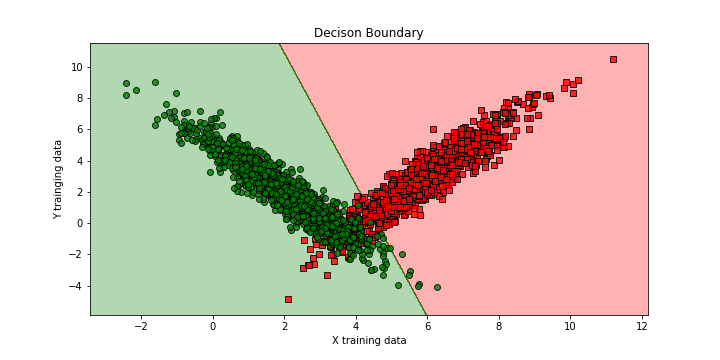
\includegraphics[scale = 0.75]{image_1.png} \\ 
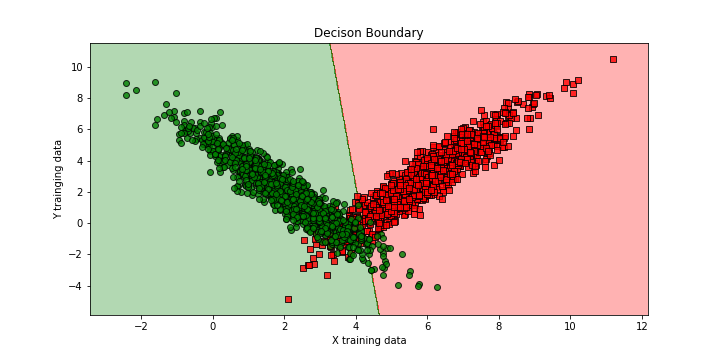
\includegraphics[scale = 0.75]{image_2.png} \\  
\newpage
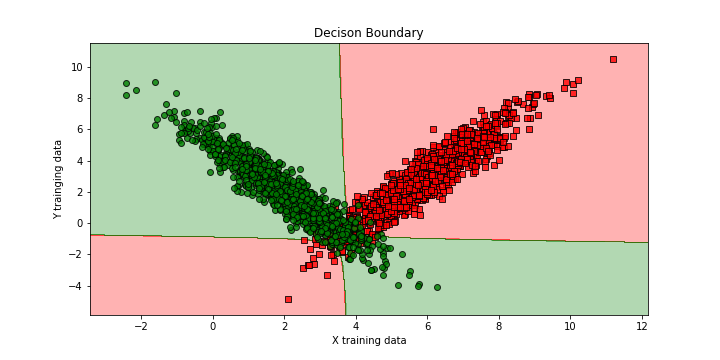
\includegraphics[scale = 0.75]{image_3.png} \\ 
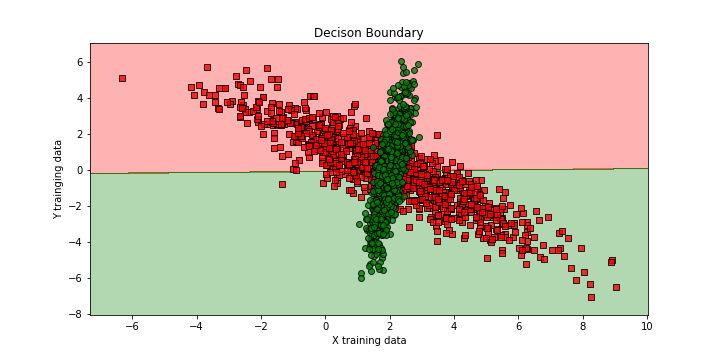
\includegraphics[scale = 0.75]{image_4.png} \\ 
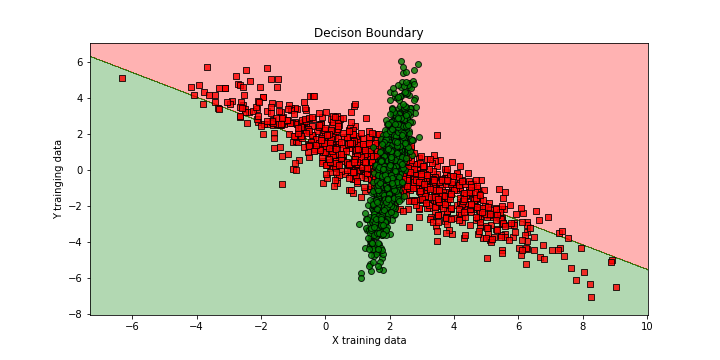
\includegraphics[scale = 0.75]{image_5.png} \\ 
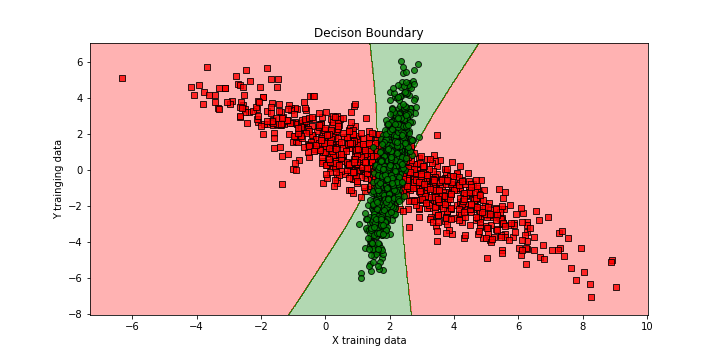
\includegraphics[scale = 0.75]{image_6.png}

\part[3] Give the ROC curves for all the classifiers. Note that a ROC curve plots the FPR (False Positive Rate) on the x-axis and TPR (True Positive Rate) on the y-axis.
\begin{solution}
\end{solution}

\part[2] Provide the error rates for the above classifiers (3 classifiers on the two datasets as $3\times2$ table, with appropriately named rows and columns).  
\begin{solution}
  In Notebook 
\end{solution}

\part[2] Summarise and explain your observations based on your plots and the assumptions given in the problem. Also briefly comment whether a non-parametric density estimation approach could have been used to solve this problem, and if so, what the associated pros/cons are compared to the parametric MLE based approach you have implemented.   
\begin{solution}
  In Notebook
\end{solution}
\end{parts}


\question[5][{\sc Coding a different density estimation?}] In the previous question, the class conditional densities were Gaussian. But not all real-world datasets are Gaussian as is to begin with. For instance, consider this data on expression/activity level of genes in the skeletal muscle tissue of different individuals, provided as a ``Genes $\times$ Samples'' matrix in this \href{https://drive.google.com/file/d/1TmVdJXqSt5yNbRr2SzyoVS2wnmXYtcos/view?usp=sharing}{link}. \\
(Note: Put all your code pertaining to this question into a single file  rollno1\_rollno2{\bf\_genes}.<fileextension>, and include this single file inside the Q6 folder of the rollno1\_rollno2.zip file mentioned in the previous question.)
\begin{parts}
\part[2] (Model Selection) How would you model any given gene in this dataset, i.e., what distribution will you assume for a gene? Assume that every gene follows the same parametric model/distribution, but with different parameter values. Support your assumption.  
\begin{solution}
\end{solution}

\part[2] (MLE Code) How will you obtain the MLE estimates of the assumed model's parameters? (no need to derive it, just state your answer as a closed-form formula or as an optimization method). Write a code to estimate these parameters for each gene.  
\begin{solution}
\end{solution}

\part[1] (Diagnostic Plots) Use your code to also plot the sample mean (x-axis) vs. sample variance (y-axis) of each gene (across all genes, with each dot in this scatter-plot being a gene). Overlay on this plot using a different color, the model mean vs. variance of each gene (i.e., mean/variance calculated using the expectation/variance formula implied by the model/distribution learnt via MLE). What does this plot tell you? 
\begin{solution}
\end{solution}
\end{parts}
\end{questions}
\end{document}